\documentclass{article}[12 pt]
\usepackage{amssymb}
\usepackage{amsthm}
\usepackage{amsmath}
\usepackage{appendix}
\usepackage{array}
\usepackage{geometry}
\usepackage{enumitem}
\usepackage{graphicx}
\usepackage{subfig}
\usepackage{caption}
\usepackage{url}
\usepackage{float}
\usepackage{pdfpages}
\usepackage{shortvrb}
\usepackage{mathtools}
\usepackage{multirow}
\usepackage{hyperref}
\usepackage{algorithm}
\usepackage[noend]{algpseudocode}
\usepackage{bm}

\def\BibTeX{{\rm B\kern-.05em{\sc i\kern-.025em b}\kern-.08em
		T\kern-.1667em\lower.7ex\hbox{E}\kern-.125emX}}

\graphicspath{{"//ece-azare-nas1.ad.ufl.edu/ece-azare-nas/Profile/cmccurley/Desktop/ImageProcessing/HW03/Report/Images/"}}
\geometry{margin=1 in}

\newcommand{\smallvskip}{\vspace{5 pt}}
\newcommand{\medvskip}{\vspace{30 pt}}
\newcommand{\bigvskip}{\vspace{100 pt}}
\newcommand{\tR}{\mathtt{R}}

%===================================================================================================================
\begin{document}
	
\begin{center}
	\textbf{\Large Connor McCurley} \\
	EEE 6512 \qquad \textbf{\large Homework 3 Due September 29, 2018} \qquad Fall 2018 
\end{center}

%===================================================================================================================
\section*{Part I Textbook Questions}

\subsection*{3.6}
\begin{itemize}
\item (a) As an example, if the LSB plane was zeroed, a few things would happen.  First, there would be no odd values in the histogram, and would therefore become more spare.  Second, each of the even histogram values would pick up their latter neighbor's value, i.e. 0's value adds with 1's, 2 with 3 and so on.  Lastly, the visual effect will be to reduce the contrast in the image.

\item (b) If instead we zero out higher-order bit planes, we get a different effect.  As another example, if we have an 8-bit image and we zero the MSB plane, the histogram will be zero for every value above 127.  Additionally, each of the values above 127 will shift and be added to smaller order values, i.e., 0+128, 1+129, and so on.  Visually, this has the effect of darkening the image.
\end{itemize}


\subsection*{3.34}

\begin{itemize}
\item (a) If the images shown are blurred with a box kernel the resulting histograms will not be the same as the originals.  The split image will retain much more of its original histogram than the checkerboard, with the exception being values on its boundary between low and high intensities.  The checkerboard image's histogram will change much more drastically, as there are many more areas of high frequency that will be blurred.  

\item (b) The extremely crude sketchs belows how the general trends of the blurred histograms. The left is the blurred histogram of the split image.  Most of the 0 and 255 pixels are retained with some being blurred along the intensity boundary.  The right resembles the histogram of the blurred checkerboard image.  Since the image has many small patches demonstrating high frequency, the resulting histogram will be more evenly distributed across the range of intensities. 
\end{itemize}

\begin{figure}[h!]
\captionsetup[subfloat]{labelformat=empty}
\centering
\subfloat[]{
  \includegraphics[width=55mm]{"SplitHist"}
}
\subfloat[]{
  \includegraphics[width=55mm]{"CheckerHist"}
}
\caption{Left: Sketch of a histogram for the blurred "split" image Right: Sketch of the histogram for the "checkerboard" image}
\end{figure}

\subsection*{3.36}
\begin{itemize}
\item (a) Yes, since the convolution of Gaussians is also Gaussian, the convolution of the three kernels will result in a Gaussian kernel. 

\item (b)  Given by Table 3.6 in the textbook, the standard deviation will be the sum of the squares of the individual kernel's standard deviations.  That is $\sigma = \sqrt{\sigma_{3}^{2}+\sigma_{5}^{2} + \sigma_{7}^{2}} = \sqrt{(1.5)^{2}+(2)^{2} + (4)^{2}} \approx 4.72 $

\item (c) The size of the resulting kernel will remain the size of the largest kernel, so 7x7.
\end{itemize}


\subsection*{3.48}
In this situation, the results would be dependent on the order the filters are applied. The effects of the second filter would be diminished by the appliaction of the first.  i.e. If blurring is done, then sharpening will not necessarily have the same effect as when sharpening before blurring is performed.


\subsection*{3.55}
\begin{itemize}
\item (a) The Laplacian kernels are not seperable.  The examples provided in the book have $rank=2$.

\item (b)  The Roberts cross-gradient kernels are not seperable.  The examples provided in the book have $rank=2$.

\item (c) The Sobel kernels shown in the book are seperable as they demonstrated $rank=1$.  Examples of the $\bm{v}$ and $\bm{w}$ whose outer product can reproduce the example kernels are $\bm{v} = [-1, 0, 1]^T$ and $\bm{w} = [1, 2, 1]^T$.  The Sobel kernel shown in Fig. 3.56(d) can be reconstructed by $\bm{v}\bm{w}^T$ and (e) by $\bm{w}\bm{v}^T$
\end{itemize}


\section*{Part II MATLAB Programming}

\section*{Part III Extra Credit}



%===================================================================================================================
% \newpage
% \section*{Part II Matlab Programming}

% \subsection*{myhist}

% \begin{figure}[h!]
% \captionsetup[subfloat]{labelformat=empty}
% \centering
% \subfloat[]{
%   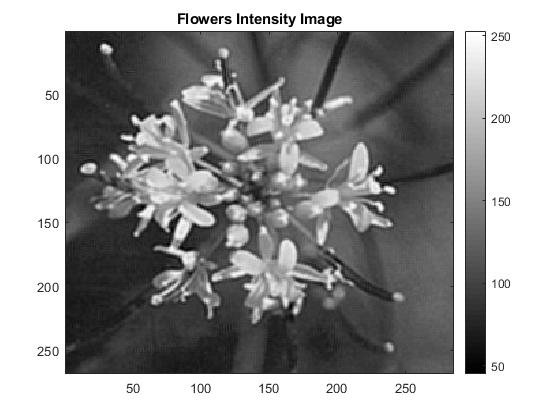
\includegraphics[width=55mm]{flowersIntensity.jpg}
% }
% \subfloat[]{
%   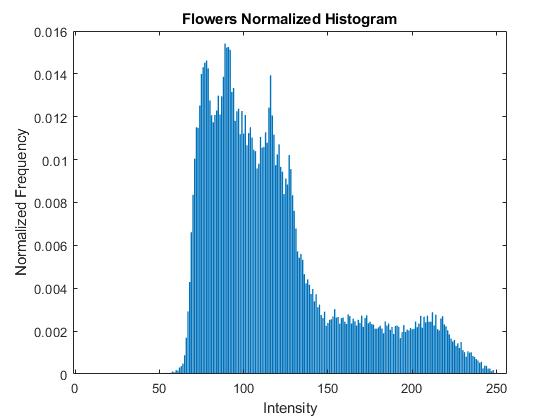
\includegraphics[width=55mm]{flowersNormHist.jpg}
% }
% \hspace{0mm}
% \subfloat[]{
%   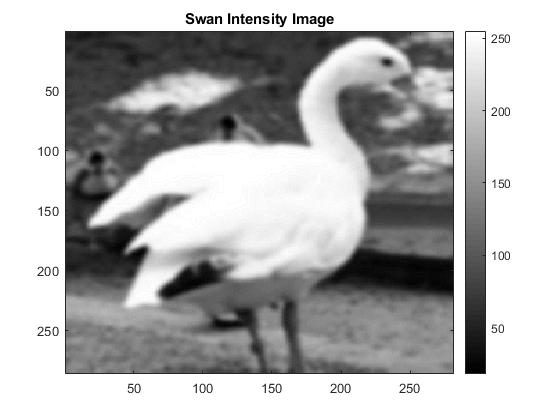
\includegraphics[width=55mm]{swanIntensity.jpg}
% }
% \subfloat[]{
%   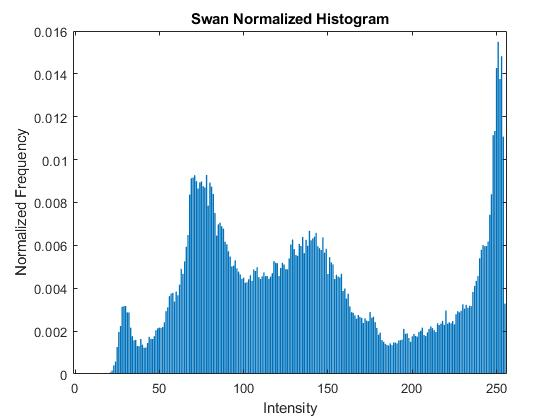
\includegraphics[width=55mm]{swanNormHist.jpg}
% }
% \hspace{0mm}
% \subfloat[]{
%   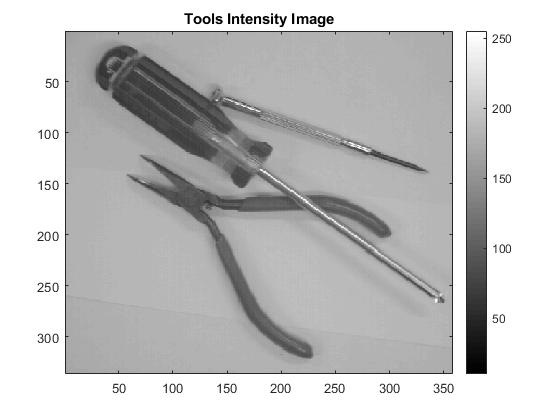
\includegraphics[width=55mm]{toolsIntensity.jpg}
% }
% \subfloat[]{
%   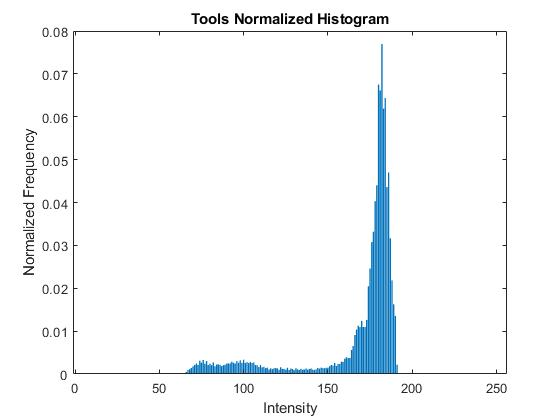
\includegraphics[width=55mm]{toolsNormHist.jpg}
% }
% \caption{Left Column: Original 8-bit Intensity Images Right Column: Normalized Histogram of Image Intensities}
% \end{figure}

% From the image histograms, the following inferences can be made about each image: 
% \begin{itemize}
% \item Flowers: Demonstrates low contrast, favors darker intensities
% \item Swan: Shows more high-contrast characteristics than the other images
% \item Tools: Exhibits low-contrast tendencies, favors lighter values
% \end{itemize}

% \newpage
% \subsection*{myhisteq}

% \begin{figure}[h!]
% \captionsetup[subfloat]{labelformat=empty}
% \centering
% \subfloat[]{
%   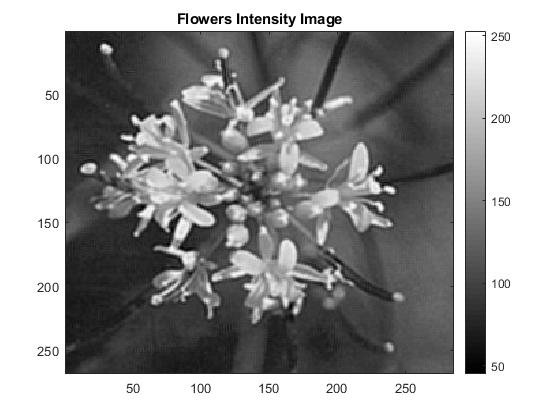
\includegraphics[width=35mm]{flowersIntensity.jpg}
% }
% \subfloat[]{
%   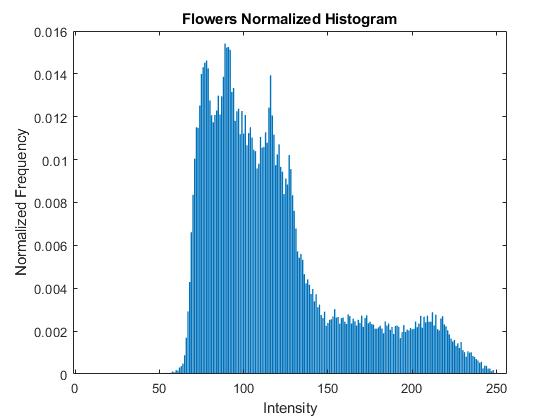
\includegraphics[width=35mm]{flowersNormHist.jpg}
% }
% \subfloat[]{
%   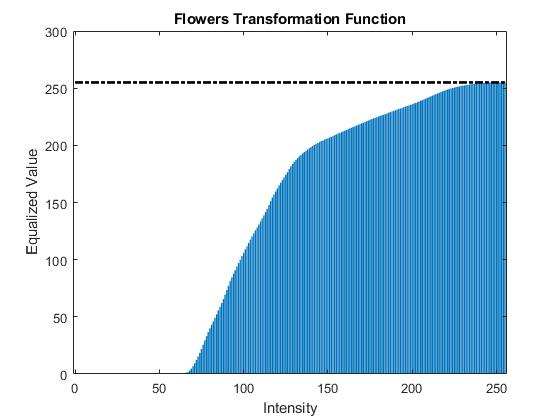
\includegraphics[width=35mm]{flowersEqTrans.jpg}
% }
% \subfloat[]{
%   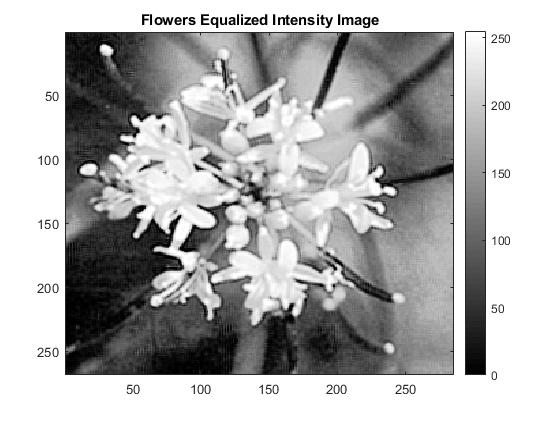
\includegraphics[width=35mm]{flowersIntensityEq.jpg}
% }
% \subfloat[]{
%   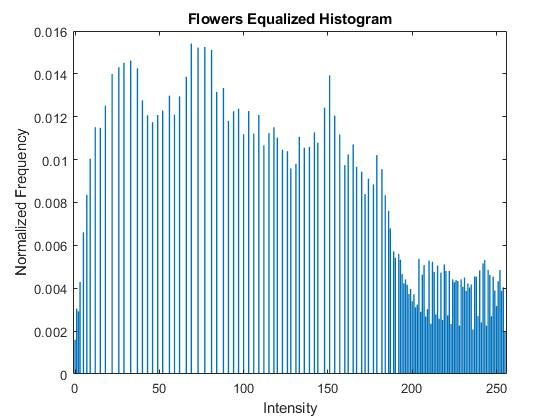
\includegraphics[width=35mm]{flowersNormHistEq.jpg}
% }
% \hspace{0mm}
% \subfloat[]{
%   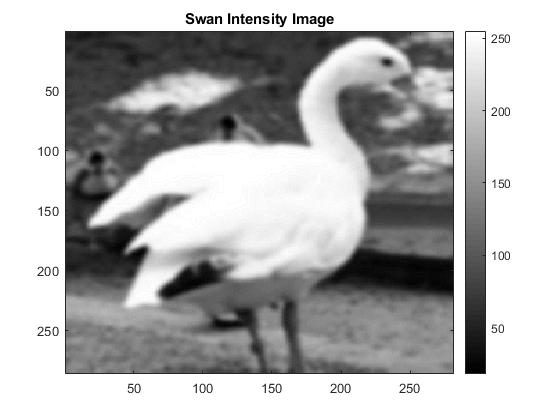
\includegraphics[width=35mm]{swanIntensity.jpg}
% }
% \subfloat[]{
%   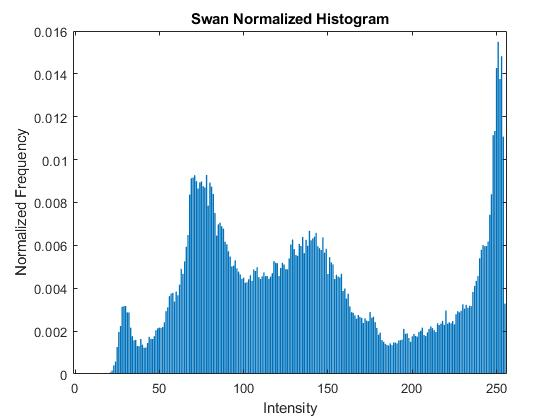
\includegraphics[width=35mm]{swanNormHist.jpg}
% }
% \subfloat[]{
%   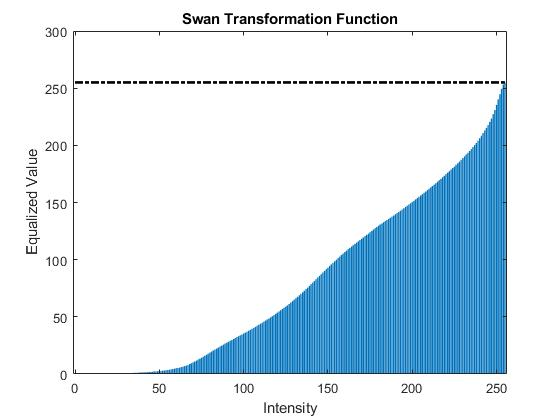
\includegraphics[width=35mm]{swanEqTrans.jpg}
% }
% \subfloat[]{
%   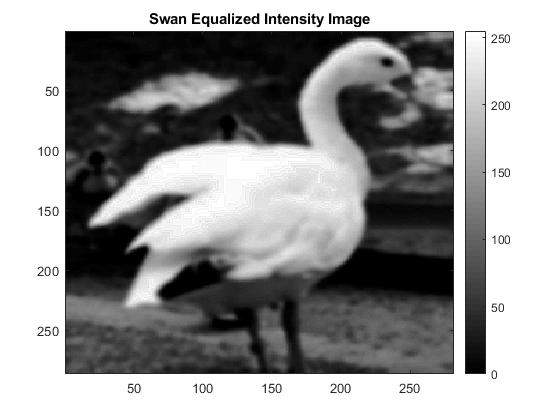
\includegraphics[width=35mm]{swanIntensityEq.jpg}
% }
% \subfloat[]{
%   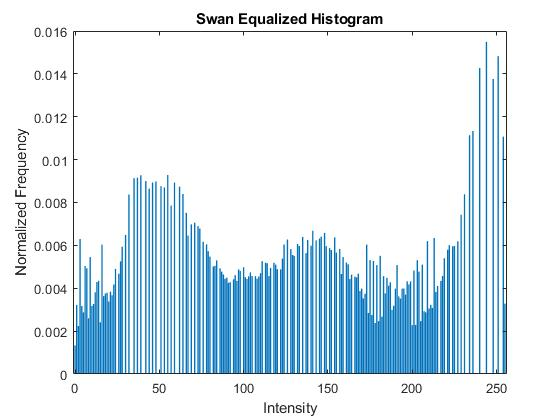
\includegraphics[width=35mm]{swanNormHistEq.jpg}
% }
% \hspace{0mm}
% \subfloat[]{
%   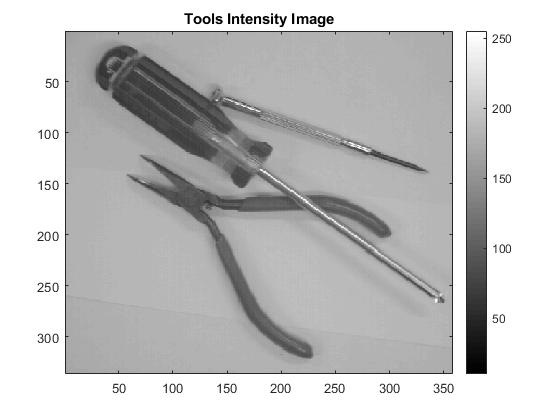
\includegraphics[width=35mm]{toolsIntensity.jpg}
% }
% \subfloat[]{
%   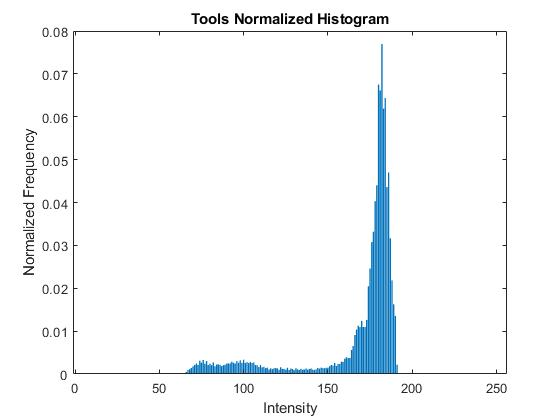
\includegraphics[width=35mm]{toolsNormHist.jpg}
% }
% \subfloat[]{
%   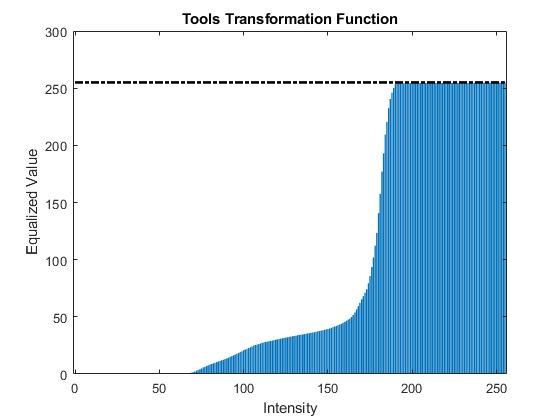
\includegraphics[width=35mm]{toolsEqTrans.jpg}
% }
% \subfloat[]{
%   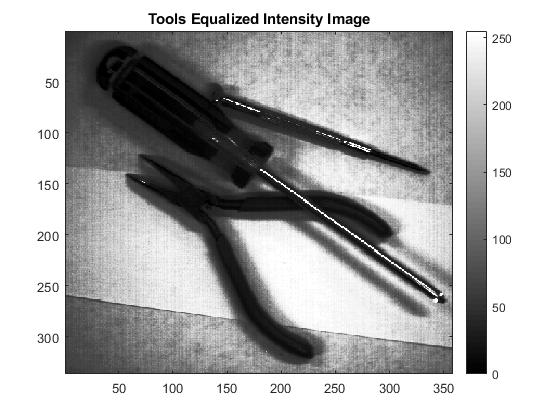
\includegraphics[width=35mm]{toolsIntensityEq.jpg}
% }
% \subfloat[]{
%   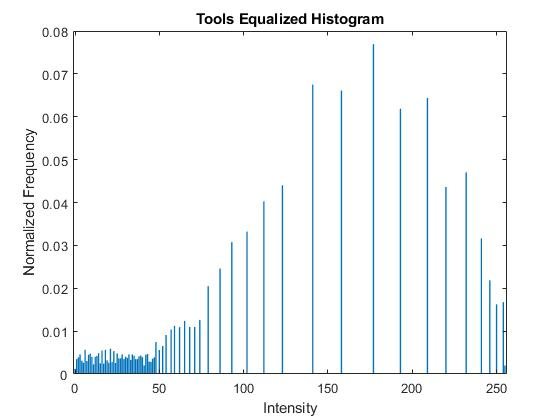
\includegraphics[width=35mm]{toolsNormHistEq.jpg}
% }
% \caption{Left to right columns: Original 8-bit Intensity Images,  Normalized Histogram of Image Intensities, Equalization Transformation Function, Equalized Intensity Image, Equalized Normalized Intensity Histogram}
% \end{figure}

% \noindent
% The above images demonstrate the outputs of the \emph{myhisteq} function required for this assignment.  The differences between the original intensity images and the equalized images transformed by the shown equalization functions can be observed visually, as well as quantitatively through the normalized image intensity histograms.

% \newpage
% \subsection*{myquantize}
% \begin{figure}[h!]
% \captionsetup[subfloat]{labelformat=empty}
% \centering
% \subfloat[]{
%   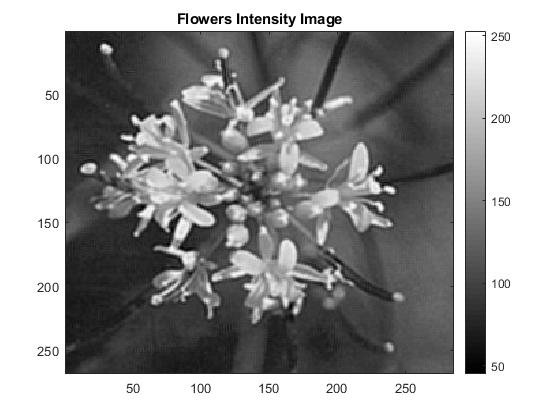
\includegraphics[width=40mm]{flowersIntensity.jpg}
% }
% \subfloat[]{
%   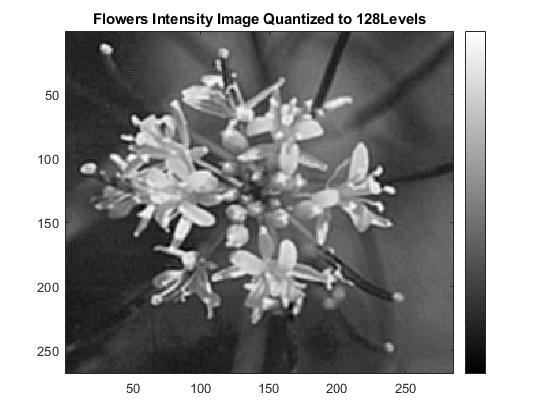
\includegraphics[width=40mm]{flowersQuant128.jpg}
% }
% \subfloat[]{
%   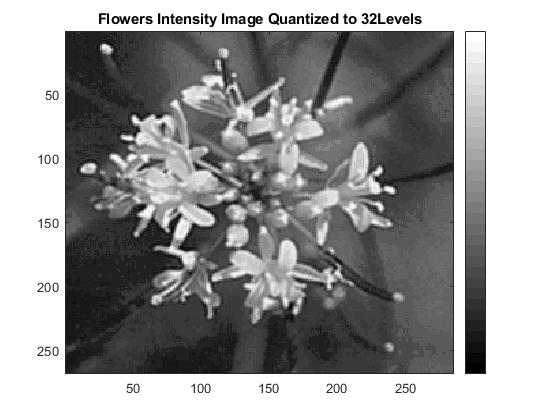
\includegraphics[width=40mm]{flowersQuant32.jpg}
% }
% \subfloat[]{
%   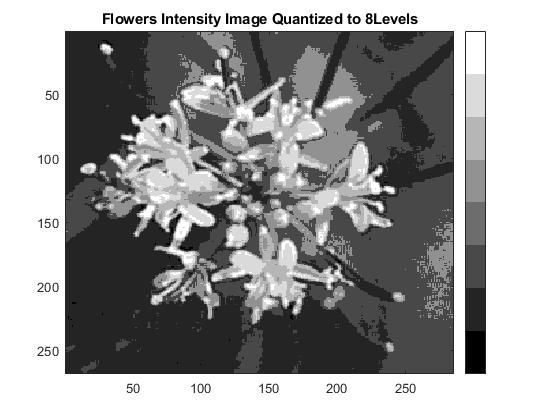
\includegraphics[width=40mm]{flowersQuant8.jpg}
% }
% \hspace{0mm}
% \subfloat[]{
%   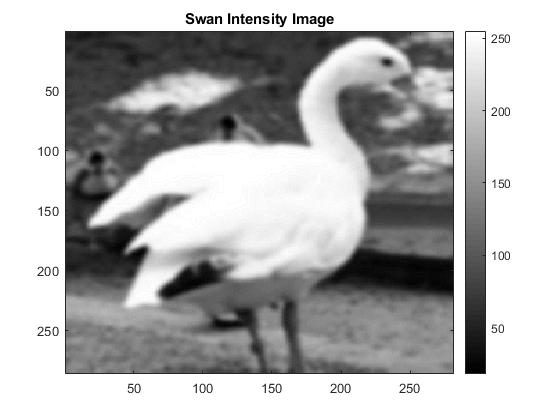
\includegraphics[width=40mm]{swanIntensity.jpg}
% }
% \subfloat[]{
%   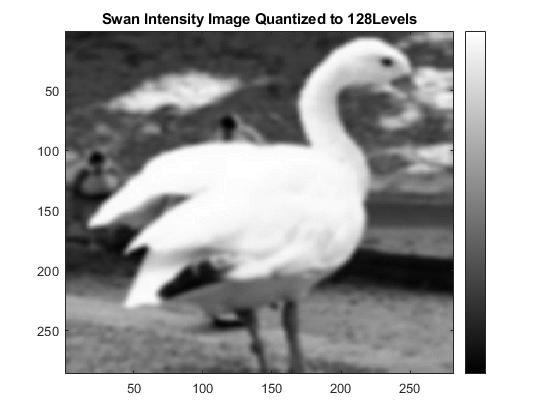
\includegraphics[width=40mm]{swanQuant128.jpg}
% }
% \subfloat[]{
%   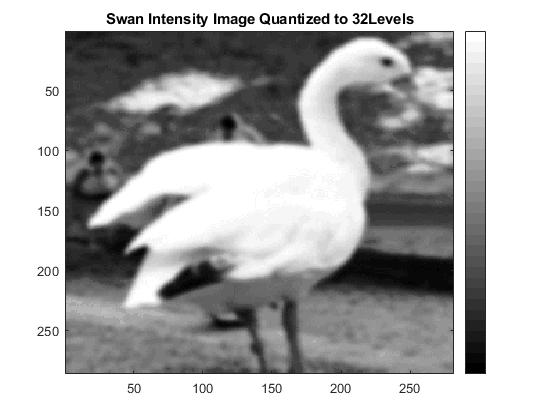
\includegraphics[width=40mm]{swanQuant32.jpg}
% }
% \subfloat[]{
%   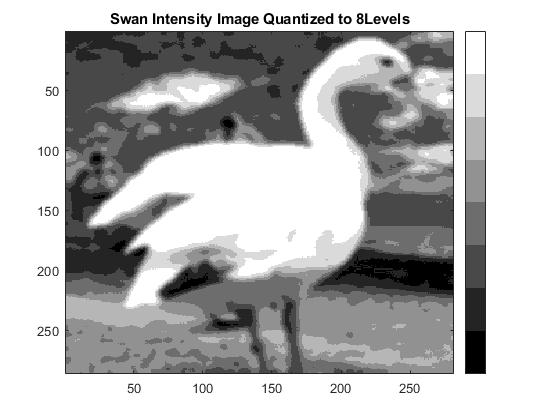
\includegraphics[width=40mm]{swanQuant8.jpg}
% }
% \hspace{0mm}
% \subfloat[]{
%   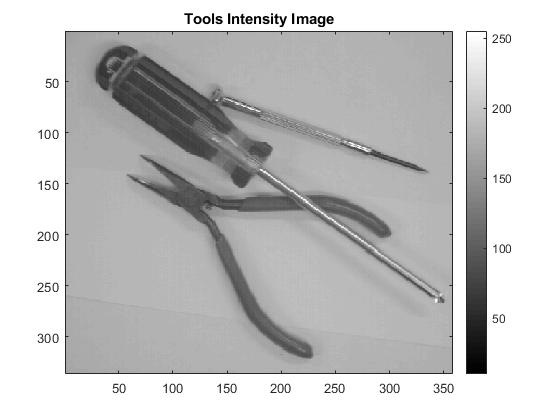
\includegraphics[width=40mm]{toolsIntensity.jpg}
% }
% \subfloat[]{
%   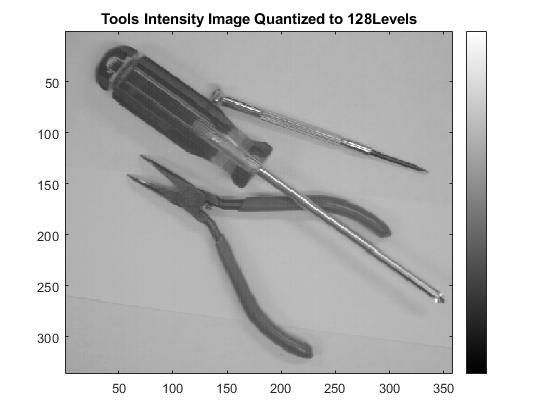
\includegraphics[width=40mm]{toolsQuant128.jpg}
% }
% \subfloat[]{
%   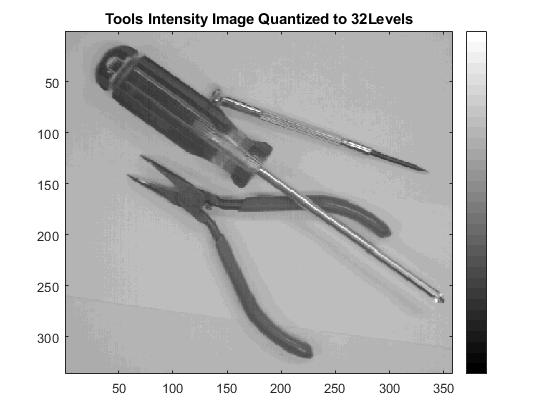
\includegraphics[width=40mm]{toolsQuant32.jpg}
% }
% \subfloat[]{
%   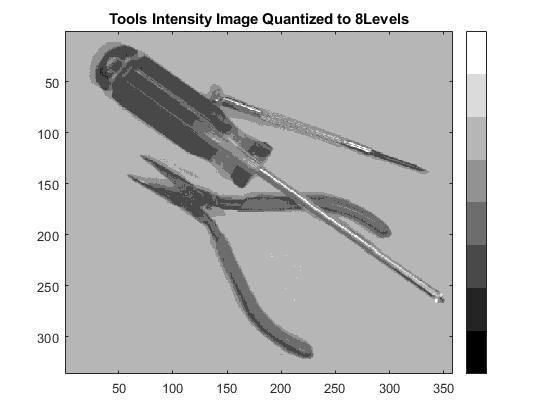
\includegraphics[width=40mm]{toolsQuant8.jpg}
% }
% \caption{From left to right: Original 8-bit Intensity image, Image quantized to 128 levels, Image quantized to 32 levels, Image quantized to 8 levels}
% \end{figure}




% \begin{algorithm}[H]
% \caption{Quantization}\label{alg:quant}
% \begin{algorithmic}[1]
% \Procedure{Quantization}{}
% \State $\textit{quantNum} \gets \text{number of intensity levels}$
% \State $f \gets \textit{pixel intensity}$
% \State $i \gets \textit{pixel index}$
% \State $\textit{Q} \gets \textit{length of quantization intervals} = \frac{255}{quantNum}$
% \For{i in numPixels}
% \State $\textit{Index of quantized value}, Q_i(f_i) \gets \textit{floor}(\frac{f_i}{Q})$
% \State $\textit{Quantized value}, Q_i(f_i) \gets Q_i(f_i)Q+\frac{Q}{2}$
% \EndFor
% \EndProcedure
% \Return{Quantized Image}
% \end{algorithmic}
% \end{algorithm}
% \vspace{5mm}
% \noindent
% The quantization function implemented for this assignment works as described in algorithm \ref{alg:quant}. \\
% \noindent
% In words, the space of possible intensities is divided into \textit{quantNum} regions.  Each pixel's intensity is classified into one of the regions.  Then each pixel's quantized value is set as the middle intensity value in its corresponding region.\\
%  %===================================================================================================================
 
%  \noindent 
%  Accompanying code is provided in $mccurleyHW02.mat$


\end{document}
